%╔════════════════════════════╗
%║	  Szablon dostosował	  ║
%║	mgr inż. Dawid Kotlarski  ║
%║		  16.10.2021		  ║
%╚════════════════════════════╝
\documentclass[12pt,twoside,a4paper,openany]{article}

    % ------------------------------------------------------------------------
% PAKIETY
% ------------------------------------------------------------------------

%różne pakiety matematyczne, warto przejrzeć dokumentację, muszą być powyżej ustawień językowych.
\usepackage{mathrsfs}   %Różne symbole matematyczne opisane w katalogu ~\doc\latex\comprehensive. Zamienia \mathcal{L} ze zwykłego L na L-transformatę.
\usepackage{eucal}      %Różne symbole matematyczne.
\usepackage{amssymb}    %Różne symbole matematyczne.
\usepackage{amsmath}    %Dodatkowe funkcje matematyczne, np. polecenie \dfac{}{} skladajace ulamek w trybie wystawionym (porównaj $\dfrac{1}{2}$, a $\frac{1}{2}$).

%język polski i klawiatura
\usepackage[polish]{babel}
%\usepackage{qtimes} % czcionka Times new Roman
\usepackage[OT4]{polski}
%\usepackage[cp1250]{inputenc}                       %Strona kodowa polskich znaków.

%obsługa pdf'a
\usepackage[pdftex,usenames,dvipsnames]{color}      %Obsługa kolorów. Opcje usenames i dvipsnames wprowadzają dodatkowe nazwy kolorow.
\usepackage[pdftex,pagebackref=false,draft=false,pdfpagelabels=false,colorlinks=true,urlcolor=blue,linkcolor=black,citecolor=green,pdfstartview=FitH,pdfstartpage=1,pdfpagemode=UseOutlines,bookmarks=true,bookmarksopen=true,bookmarksopenlevel=2,bookmarksnumbered=true,pdfauthor={Dawid Kotlarski},pdftitle={Praca Inznierska},pdfsubject={},pdfkeywords={transient recovery voltage trv},unicode=true]{hyperref}   %Opcja pagebackref=true dotyczy bibliografii: pokazuje w spisie literatury numery stron, na których odwołano się do danej pozycji.
\usepackage{hyperref}
%bibliografia
%\usepackage[numbers,sort&compress]{natbib}  %Porządkuje zawartość odnośników do literatury, np. [2-4,6]. Musi być pod pdf'em, a styl bibliogfafii musi mieć nazwę z dodatkiem 'nat', np. \bibliographystyle{unsrtnat} (w kolejności cytowania).
\usepackage[
backend=bibtex,
style=numeric,
sorting=none
]{biblatex}
\addbibresource{bibliografia.bib}
\usepackage{hypernat}                       %Potrzebna pakietowi natbib do wspolpracy z pakietem hyperref (wazna kolejnosc: 1. hyperref, 2. natbib, 3. hypernat).

%grafika i geometria strony
\usepackage{extsizes}           %Dostepne inne rozmiary czcionek, np. 14 w poleceniu: \documentclass[14pt]{article}.
\usepackage[final]{graphicx}
\usepackage[a4paper,left=3.5cm,right=2.5cm,top=2.5cm,bottom=2.5cm]{geometry}

%strona tytułowa
\usepackage{strona_tytulowa}

%inne
\usepackage[hide]{todo}                     %Wprowadza polecenie \todo{treść}. Opcje pakietu: hide/show. Polecenie \todos ma byc na koncu dokumentu, wszystkie \todo{} po \todos sa ignorowane.
\usepackage[basic,physics]{circ}            %Wprowadza środowisko circuit do rysowania obwodów elektrycznych. Musi byc poniżej pakietow językowych.
\usepackage[sf,bf,outermarks]{titlesec}     %Troszczy się o wygląd tytułów rozdziałów (section, subsection, ...). sf oznacza czcionkę sans serif (typu arial), bf -- bold. U mnie: oddzielna linia dla naglowku paragraph. Patrz tez: tocloft -- lepiej robi format spisu tresci.
\usepackage{tocloft}                        %Troszczy się o format spisu trsci.
\usepackage{expdlist}    %Zmienia definicję środowiska description, daje większe możliwości wpływu na wygląd listy.
\usepackage{flafter}     %Wprowadza parametr [tb] do polecenia \suppressfloats[t] (polecenie to powoduje nie umieszczanie rysunkow, tabel itp. na stronach, na ktorych jest to polecenie (np. moze byc to stroma z tytulem rozdzialu, ktory chcemy zeby byl u samej gory, a nie np. pod rysunkiem)).
\usepackage{array}       %Ładniej drukuje tabelki (np. daje wiecej miejsca w komorkach -- nie są tak ścieśnione, jak bez tego pakietu).
\usepackage{listings}    %Listingi programow.
\usepackage[format=hang,labelsep=period,labelfont={bf,small},textfont=small]{caption}   %Formatuje podpisy pod rysunkami i tabelami. Parametr 'hang' powoduje wcięcie kolejnych linii podpisu na szerokosc nazwy podpisu, np. 'Rysunek 1.'.
\usepackage{appendix}    %Troszczy się o załączniki.
\usepackage{floatflt}    %Troszczy się o oblewanie rysunkow tekstem.
\usepackage{here}        %Wprowadza dodtkowy parametr umiejscowienia rysunków, tabel, itp.: H (duże). Umiejscawia obiekty ruchome dokladnie tam gdzie są w kodzie źródłowym dokumentu.
\usepackage{makeidx}     %Troszczy się o indeks (skorowidz).

%nieużywane, ale potencjalnie przydatne
\usepackage{sectsty}           %Formatuje nagłówki, np. żeby były kolorowe -- polecenie: \allsectionsfont{\color{Blue}}.
%\usepackage{version}           %Wersje dokumentu.

%============
\usepackage{longtable}			%tabelka
%============


%PAGINA GÓRNA I DOLNA
\usepackage{fancyhdr}          %Dodaje naglowki jakie się chce.
\pagestyle{fancy}
\fancyhf{}
% numery stron w paginie dolnej na srodku
\fancyfoot[C]{\scriptsize DOKUMENTACJA PROJEKTU - INŻYNIERIA OPROGRAMOWANIA \\ 
\normalsize\sffamily  \thepage}


%\fancyhead[L]{\small\sffamily \nouppercase{\leftmark}}
\fancyhead[C]{\footnotesize \textit{AKADEMIA NAUK STOSOWANYCH W NOWYM SĄCZU}\\}

\renewcommand{\headrulewidth}{0.4pt}
\renewcommand{\footrulewidth}{0.4pt}

    % ------------------------------------------------------------------------
% USTAWIENIA
% ------------------------------------------------------------------------

% ------------------------------------------------------------------------
%   Kropki po numerach sekcji, podsekcji, itd.
%   Np. 1.2. Tytuł podrozdziału
% ------------------------------------------------------------------------
\makeatletter
    \def\numberline#1{\hb@xt@\@tempdima{#1.\hfil}}                      %kropki w spisie treści
    \renewcommand*\@seccntformat[1]{\csname the#1\endcsname.\enspace}   %kropki w treści dokumentu
\makeatother

% ------------------------------------------------------------------------
%   Numeracja równań, rysunków i tabel
%   Np.: (1.2), gdzie:
%   1 - numer sekcji, 2 - numer równania, rysunku, tabeli
%   Uwaga ogólna: o otoczeniu figure ma być najpierw \caption{}, potem \label{}, inaczej odnośnik nie działa!
% ------------------------------------------------------------------------
\makeatletter
    \@addtoreset{equation}{section} %resetuje licznik po rozpoczęciu nowej sekcji
    \renewcommand{\theequation}{{\thesection}.\@arabic\c@equation} %dodaje kropki

    \@addtoreset{figure}{section}
    \renewcommand{\thefigure}{{\thesection}.\@arabic\c@figure}

    \@addtoreset{table}{section}
    \renewcommand{\thetable}{{\thesection}.\@arabic\c@table}
\makeatother

% ------------------------------------------------------------------------
% Tablica
% ------------------------------------------------------------------------
\newenvironment{tabela}[3]
{
    \begin{table}[!htb]
    \centering
    \caption[#1]{#2}
    \vskip 9pt
    #3
}{
    \end{table}
}

% ------------------------------------------------------------------------
% Dostosowanie wyglądu pozycji listy \todos, np. zamiast 'p.' jest 'str.'
% ------------------------------------------------------------------------
\renewcommand{\todoitem}[2]{%
    \item \label{todo:\thetodo}%
    \ifx#1\todomark%
        \else\textbf{#1 }%
    \fi%
    (str.~\pageref{todopage:\thetodo})\ #2}
\renewcommand{\todoname}{Do zrobienia...}
\renewcommand{\todomark}{~uzupełnić}

% ------------------------------------------------------------------------
% Definicje
% ------------------------------------------------------------------------
\def\nonumsection#1{%
    \section*{#1}%
    \addcontentsline{toc}{section}{#1}%
    }
\def\nonumsubsection#1{%
    \subsection*{#1}%
    \addcontentsline{toc}{subsection}{#1}%
    }
\reversemarginpar %umieszcza notki po lewej stronie, czyli tam gdzie jest więcej miejsca
\def\notka#1{%
    \marginpar{\footnotesize{#1}}%
    }
\def\mathcal#1{%
    \mathscr{#1}%
    }
\newcommand{\atp}{ATP/EMTP} % Inaczej: \def\atp{ATP/EMTP}

% ------------------------------------------------------------------------
% Inne
% ------------------------------------------------------------------------
\frenchspacing                      
\hyphenation{ATP/-EMTP}             %dzielenie wyrazu w danym miejscu
\setlength{\parskip}{3pt}           %odstęp pomiędzy akapitami
\linespread{1.3}                    %odstęp pomiędzy liniami (interlinia)
\setcounter{tocdepth}{4}            %uwzględnianie w spisie treści czterech poziomów sekcji
\setcounter{secnumdepth}{4}         %numerowanie do czwartego poziomu sekcji 
\titleformat{\paragraph}[hang]      %wygląd nagłówków
{\normalfont\sffamily\bfseries}{\theparagraph}{1em}{}



    %polecenia zdefiniowane w pakiecie strona_tytulowa.sty
    \title{Aplikacja Quizowa "BrainCell"}	
    \author{Dariusz Łopian}
    \authorI{Motyka Szymon}
    \authorII{Matras Szymon}		%jeśli są dwie osoby w projekcie to zostawiamy:    \authorII{}
		
	\uczelnia{AKADEMIA NAUK STOSOWANYCH \\W NOWYM SĄCZU}
    \instytut{Wydział Nauk Inżynieryjnych}
    \kierunek{Informatyka Stosowana}
    \praca{DOKUMENTACJA PROJEKTOWA}
    \przedmiot{Inżynieria Oprogramowania}
    \prowadzacy{mgr inż. Daniel Drozd}
    \rok{2022}


%definicja składni mikrotik
\usepackage{fancyvrb}
\DefineVerbatimEnvironment{MT}{Verbatim}%
{commandchars=\+\[\],fontsize=\small,formatcom=\color{red},frame=lines,baselinestretch=1,} 
\let\mt\verb 
%zakonczenie definicji składni mikrotik

\usepackage{fancyhdr}    %biblioteka do nagłówka i stopki

			
\begin{document}
   
    \renewcommand{\figurename}{Rys.}    %musi byc pod \begin{document}, bo w~tym miejscu pakiet 'babel' narzuca swoje ustawienia
    \renewcommand{\tablename}{Tab.}     %j.w.
    \thispagestyle{empty}               %na tej stronie: brak numeru
    \stronatytulowa                     %strona tytułowa tworzona przez pakiet strona_tytulowa.tex
 
 \pagestyle{fancy}

    \newpage

    %formatowanie spisu treści i~nagłówków
    \renewcommand{\cftbeforesecskip}{8pt}
    \renewcommand{\cftsecafterpnum}{\vskip 8pt}
    \renewcommand{\cftparskip}{3pt}
    \renewcommand{\cfttoctitlefont}{\Large\bfseries\sffamily}
    \renewcommand{\cftsecfont}{\bfseries\sffamily}
    \renewcommand{\cftsubsecfont}{\sffamily}
    \renewcommand{\cftsubsubsecfont}{\sffamily}
    \renewcommand{\cftparafont}{\sffamily}
    %koniec formatowania spisu treści i nagłówków
     
    \tableofcontents    %spis treści
    \thispagestyle{fancy}
    \newpage

    
    \newpage

    
%%%%%%%%%%%%%%%%%%% treść główna dokumentu %%%%%%%%%%%%%%%%%%%%%%%%%

   	\newpage
\section{Opis i cel projektu}		%1
Aplikacja \textbf{BrainCell} to gra mobilna oparta o aplikacje typu quiz, w którym mamy za zadanie wybrać jedną prawidłową odpowiedź z czterech podanych. Dzięki temu, że aplikacja będzie napisana na telefony komórkowe z systemem android, uzyskamy możliwość sprawdzenia swojego poziomu wiedzy w dowolnym miejscu. Użytkownik po zalogowaniu będzie miał dostęp do podglądu kategorii w jakich chce odpowiadać na pytania a przez to baza pytań będzie zawężona. Gra będzie skierowana do wszystkich użytkowników zarówno młodych, jak i starszych, ponieważ poziom pytań będzie bardzo zróżnicowany. Interfejs i obsługa będzie prosta i intuicyjna dzieki czemu nikt nie bedzię miał problemu z poruszaniem się po menu oraz po samej rozgrywce. 
\\Po wejściu do aplikacji naszym oczom ukaże się ekran logowania. Po poprawnym zalogowaniu uzyskamy widok głównego menu, w którym znajdziemy:
\\- Profil użytkownika - z poziomu którego będzie można dokonywać edycji naszych danych
\\- Wybór kategorii pytań
\\- Osiągnięcia
\\- Ustawienia
\newline Rozgrywka będzię kontrolowana przez czas. Po wybraniu interesującej nas kategorii ujrzymy pytanie oraz cztery odpowiedzi, z których jedna będzie poprawna. W górnej części ekranu zostanie wyświetlony timer, który będzie odliczał czas. Po upływie ustalonego czasu i nie zaznaczeniu żadnej odpowiedzi przez użytkownika, zostanie ona uznana jako błędna. Następnie na ekranie zostanie wyświetlone kolejne pytanie.
\newline Szata graficzna aplikacji będzie prosta, czytelna i schludna, dzieki czemu rozgrywka będzie przyjemna.


   	\newpage
\section{Wymagania funkcjonalne i niefunkcjonalne}		%2

\textbf{a) Wymagania funkcjonalne:}
\newline - Możliwość utworzenia konta i zalogowania się do aplikacji
\newline - Możliwość edycji danych w profilu użytkownika
\newline - Możliwość wyboru kategorii pytań 
\newline - Możliwość wyboru i zaznaczenie odpowiedzi na zadane pytanie
\newline - Możliwość sprawdzenia poprawnej odpowiedzi 
\newline - Możliwość weryfikacji swoich osiągnięć w grze
\newline - Możliwość zmiany motywu aplikacji w ustawieniach ( ?? )
\newline\newline\textbf{b) Wymagania niefunkcjonalne:}
\newline Po wdrożeniu większości powyższych wymagań funkcjonalnych, powinniśmy otrzymać wymagania niefunkcjonalne, takie jak:
\newline - Przejrzysta i responsywna aplikacja mobilna dla użytkowników 
\newline - Czytelny i prosty w obsłudze interfejs

   	\newline\newline
\section{Opis technologii}		%3
Podczas realizacji projektu wykorzystamy takie technologie jak:
\\ - \textbf{\textit{Flutter}} - jest to framework stworzony przez Google, za pomocą którego można tworzyć aplikacje mobilne na urządzenia z systemem Android oraz iOS. Narzędzie to rozwija się dość dynamicznie, ponieważ skupia wokół siebie dużą część społeczności programistów, dzięki łatwej i przyspieszonej pracy, a także pozwala osiągnąć zamierzone efekty przy zaangażowaniu mniejszej liczby programistów i niższych kosztach.
\\ - \textbf{\textit{C++}} - jest to jeden z bardziej popularnych języków programowania ogólnego przeznaczenia. Stosuje różne style programowania, dzięki czemu nadaje się do tworzenia systemów operacyjnych, systemów wbudowanych, aplikacji desktopowych, serwerów, czy silników gier. 
\\ - \textbf{\textit{Firebase}} - należąca do Google platforma umożliwiająca tworzenie aplikacji mobilnych oraz internetowych, wyposażona dodatkowo w bazę danych.

   	\newpage
\section{Identyfikacja problemów oraz proponowane rozwiązania}		%4
Naszym największym problemem do rozwiązania przy tworzeniu aplikacji będzie stworzenie bazy pytań wraz z odpowiadającymi im kategoriami.
Rozwiązaniem problemu może okazać się skorzystanie z gotowej już bazy pytań. 
       \newpage
\section{Diagram przypadków użycia}		%5

%rysunek
\begin{figure}[!htb]
	\begin{center}
		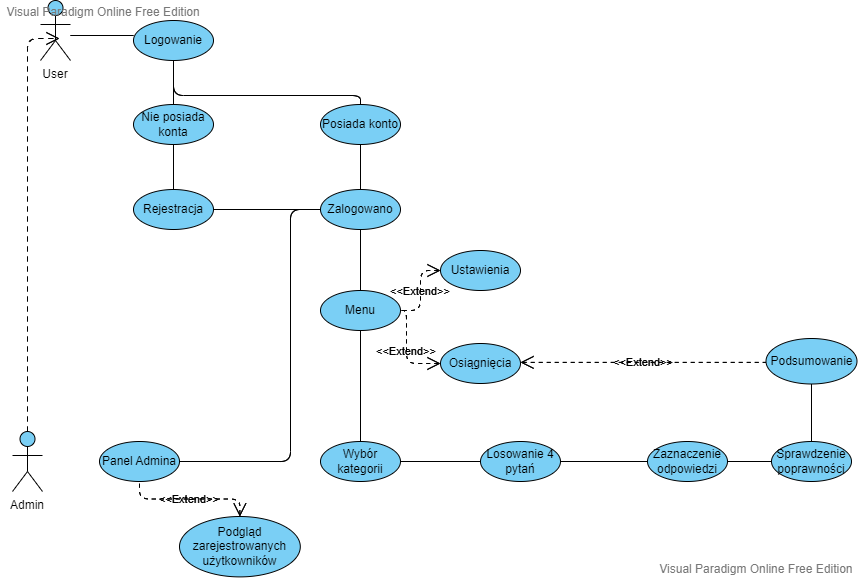
\includegraphics[width=15cm]{rys/przypadki uzycia.png}
		\caption{Diagram przypadków użycia 'BrainCell'}
		\label{rys:rysunek001}
	\end{center}
\end{figure} 
   	\newpage
\section{Scenariusze przypadków użycia}  %6
\textbf{a) Scenariusze użytkownika.}
\newline \textit{\underline{Scenariusz nr 1}}
\newline \textbf{Tytuł:} Logowanie
\newline \textbf{Warunek wejścia:} Posiada konto
\newline \textbf{Przebieg:} Użytkownik podejmuje próbę logowania. Podaje niezbędne dane (login, hasło).  
\newline \textbf{Zakończenie:} Jeśli próba logowania jest pozytywna - zyskuje dostęp do pełnej funkcjonalności aplikacji, w przeciwnym razie dostaje kolejną możliwość wprowadzenia danych logowania.
\newline \textbf{Zakończenie alternatywne:} Jeśli użytkownik nie posiada konta dostanie możliwość wykonania scenariusza nr 2 (Rejestracja).
\newline\newline \textit{\underline{Scenariusz nr 2}}, 
\newline \textbf{Tytuł:} Rejestracja
\newline \textbf{Warunek wejścia:} Musi wejść do aplikacji (kliknąć w ikonę aplikacji).
\newline \textbf{Przebieg:} Użytkownik dostaje możliwość stworzenia swojego profilu, które jest konieczne do skorzystania z aplikacji.
\newline \textbf{Zakończenie:} Jeśli rejestracja przebiegnie pomyślnie użytkownik dostanie możliwość zalogowania się do aplikacji.
\newline \textbf{Zakończenie alternatywne:} W przypadku podania błędnych danych nastąpi wyświetlenie komunikatu błędu i możliwość podjęcia kolejnej próby.
\newline\newline \textit{\underline{Scenariusz nr 3}}
\newline \textbf{Tytuł:} Edycja profilu
\newline \textbf{Warunek wejścia:} Użytkownik jest zalogowany.
\newline \textbf{Przebieg:} Użytkownik dostaje możliwość edycji profilu tzn. m. in. zmiany swojego hasła.
\newline \textbf{Zakończenie:} Po poprawnej edycji danych następuje ich zmiana.
\newline\newline \textit{\underline{Scenariusz nr 4}}
\newline \textbf{Tytuł:} Sprawdzenie osiągnięć
\newline \textbf{Warunek wejścia:} Użytkownik jest zalogowany i znajduje się w głównym menu.
\newline \textbf{Przebieg:} Użytkownik w menu głównym klika w Osiągnięcia.
\newline \textbf{Zakończenie:} Po kliknięciu następuje przejście do widoku osiągnięć, gdzie użytkownik ma możliwość sprawdzenia swoich statystyk.
\newline\newline \textit{\underline{Scenariusz nr 5}}
\newline \textbf{Tytuł:} Wybór kategorii pytań
\newline \textbf{Warunek wejścia:} Użytkownik jest zalogowany i znajduje się w głównym menu.
\newline \textbf{Przebieg:} Użytkownik w menu głównym klika w Kategorie pytań.
\newline \textbf{Zakończenie:} Po kliknięciu następuje przejście do widoku kategorii pytań z danej dziedziny wiedzy, gdzie użytkownik wybiera kategorie z jakiej chce odpowiadać.
\newline \textbf{Zakończenie alternatywne:} Użytkownik chcąc wyjść z danej kategorii klika przycisk wstecz i wychodzi do głównego menu. 


\textbf{b) Scenariusze administratora.}
\newline \textit{\underline{Scenariusz nr 1}}
\newline \textbf{Tytuł:} Logowanie
\newline \textbf{Warunek wejścia:} brak
\newline \textbf{Przebieg:} Administrator loguje się do systemu, dzięki czemu zyskuje dostęp do pełnej funkcjonalności i funkcji administratorskich.
\newline \textbf{Zakończenie:} Zalogowanie do konta oraz możliwość zarządzania poszczególnymi częściami serwisu.


   
       
%%%%%%%%%%%%%%%%%%% koniec treść główna dokumentu %%%%%%%%%%%%%%%%%%%%%
%%% ABY WYKORZYSTAĆ SEKCJE USUŃ KOMENTARZE !!!
	%	\newpage
 %   \addcontentsline{toc}{section}{Literatura}  
 %	\printbibliography
	
	

    \newpage

    \hypersetup{linkcolor=black}
    \renewcommand{\cftparskip}{3pt}
    \clearpage
    \renewcommand{\cftloftitlefont}{\Large\bfseries\sffamily}
    \listoffigures
    \addcontentsline{toc}{section}{Spis rysunków}
	\thispagestyle{fancy}
    \newpage


	


    %lista rzeczy do zrobienia: wypisuje na koñcu dokumentu, patrz: pakiet todo.sty
    \todos
    %koniec listy rzeczy do zrobienia
\end{document}
